\documentclass[11pt, oneside]{article}   	% use "amsart" instead of "article" for AMSLaTeX format
\usepackage{geometry}                		% See geometry.pdf to learn the layout options. There are lots.
\geometry{letterpaper}                   		% ... or a4paper or a5paper or ... 
%\geometry{landscape}                		% Activate for for rotated page geometry
%\usepackage[parfill]{parskip}    		% Activate to begin paragraphs with an empty line rather than an indent
\usepackage{graphicx}				% Use pdf, png, jpg, or eps§ with pdflatex; use eps in DVI mode
								% TeX will automatically convert eps --> pdf in pdflatex		
\usepackage{amssymb}

\usepackage{pgf}
\usepackage{tikz}
\usetikzlibrary{arrows,automata}
\usepackage[latin1]{inputenc}
\usepackage{verbatim}
\usetikzlibrary{automata,positioning}

\begin{document}
\noindent Gavin Grob
\\CS 510 Automata Theory
\\Homework 5
\\
\\
\\1. If $A$ and $B$ are languages define $A \diamond B$ = $\{xy | x \in A$ and $y \in B$ and $| x | = | y | \}$
\\Show that if $A$ and $B$ are regular languages then $A  \diamond  B$ is a CFL.
\\
\\I will create a PDA and call it $P$, that will recognize $A \diamond B$ to show that it is a CFL, because CFL's and PDA's are equivalent. Since we are assuming $A$ and $B$ are regular they both have DFA that define all the string in $A_{DFA}$ and $B_{DFA}$ respectively. If it was just $A_{DFA}$ and $B_{DFA}$ concatenated we would know that it would be regular under the closure property, but we have to make sure that $| x | = | y |$. So we must push $x$ onto the stack, but instead of the string $x$ I'll just make it easier and push a $C$ on the stack for every character of $x$ is read. Then while reading a character of $y$ we pop, and check to see if it is a $C$ or $Z_0$. If $C$, then we continue reading $y$. If we are in the accepting state of $B_{DFA}$, and $Z_0$ is popped, then we go to the final state of $P$.
\\
\\Here is a ROUGH idea how the new PDA will will work. It will start by pushing on $Z_0$. Then it will run through the DFA defined by $A_{DFA}$, when in the accepting state of $A$($q_{af}$) it will nondeterministicly jump to the start $q_{bs}$, where it will run till it runs into the empty stack where it goes to the final state of the PDA.
\\
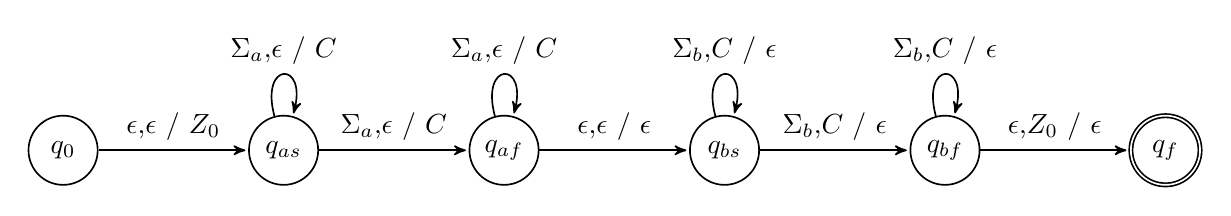
\begin{tikzpicture}[->,>=stealth',shorten >=1pt,auto,node distance=2.8cm,
                    semithick]

  \node[state] 	    (0)                   {$q_0$};
  \node[state]         (1) [right of=0] {$q_{as}$};
  \node[state]         (2) [right of=1] {$q_{af}$};
  \node[state]         (3) [right of=2] {$q_{bs}$};
  \node[state]         (4) [right of=3] {$q_{bf}$};
  \node[accepting, state]         (5) [right of=4] {$q_f$};


  \path (0) 		edge              	    node {$\epsilon$,$\epsilon$ / $Z_0$} (1)
        (1)		edge [loop above] node {$\Sigma_a$,$\epsilon$ / $C$} (1)        
        			edge              node {$\Sigma_a$,$\epsilon$ / $C$} (2)
        (2)edge [loop above] node {$\Sigma_a$,$\epsilon$ / $C$} (2)  
            edge              node {$\epsilon$,$\epsilon$ / $\epsilon$} (3)
        (3) 		edge              	    node {$\Sigma_b$,$C$ / $\epsilon$} (4)
        			edge [loop above] node {$\Sigma_b$,$C$ / $\epsilon$} (3)
        (4)		edge [loop above] node {$\Sigma_b$,$C$ / $\epsilon$} (4)        
        			edge              node {$\epsilon$,$Z_0$ / $\epsilon$} (5)
        (5)  
        ;
\end{tikzpicture}
\\
\\Formally we have a DFA repersenting the regular language $A$ we will define as:
\\$A_{DFA}$ = ($Q_a,\Sigma_a, \delta_a,q_{0a},F_a$) 
\\
\\We also have a DFA repersenting the regular language $B$ we will define as:
\\$B_{DFA}$ = ($Q_b,\Sigma_b, \delta_b,q_{0b},F_b$) 
\\
\\I will define a PDA that accepts $A \diamond B$ defined as:
\\P = ($Q,\Sigma,\Gamma, \delta,q_0,Z_0,F$)
\\
\\The states will be a new $q_0$ (used to put the bottom of the stack symbol) a new final state to detect the bottom of the stack. Then all the states from $A_{DFA}$ and $B_{DFA}$.
\\$Q = \{q_0, q_f\} \cup Q_a \cup Q_b$
\\
\\The alphabet will be all the characters from language A, and B.
\\$\Sigma = \Sigma_a \cup \Sigma_b$
\\
\\The only thing that will be on the stack is $C$ which is our count of $x$ and the bottom of the stack symbol($Z_0$).
\\$\Gamma = \{C, Z_0\}$
\\
\\$\delta(q,a,X) = $
\\
\\\{$q_{0a}, Z_0 | q = q_0, a = \epsilon, X = \epsilon\}$ 
\\move from the start state to $A_{DFA}$'s start state, while reading no input, nothing off the stack, and pushing $Z_0$
\\
\\$\{\delta_a(q,a), C | q \in Q_a, a \in \Sigma_a, X = \epsilon\}$
\\move threw $A_{DFA}$ while reading input characters in the language of $A$, nothing off the stack, and pushing $C$
\\
\\$\{q_0b,\epsilon | q \in F_a,  a = \epsilon, X = \epsilon\}$ 
\\move from a final state of $A_{DFA}$ to the start state of $B_{DFA}$, while reading no input, nothing off the stack, and pushing nothing
\\
\\$\{\delta_b(q,a), C | q \in Q_b, a \in \Sigma_b, X = C\}$
\\move threw $B_{DFA}$ while reading input characters in the language of $B$, $C$ on the stack, and popping $C$
\\
\\$\{q_f,\epsilon | q \in F_b, a = \epsilon, X = Z_0\}$ 
\\move from $B_{DFA}$'s final state to the final state, while reading no input characters, $Z_0$ on the stack, and popping $Z_0$
\\
\\
\\The new starting symbol.
\\$q_0 = q_0$
\\
\\Bottom of stack character.
\\$Z_0 = Z_0$
\\
\\The only accepting state is the new final state we created.
\\$F = \{q_f\}$
\\
\\
\\
\\2. Lets define a $perfect$ $shuffle$ of two languages $A$ and $B$ as:
\\$\{ w | w$ = $a_1b_1a_2b_2 ... a_kb_k$ where $a_1a_2 ... a_k \in A$ and $b_1b_2 ... b_k \in B \}$
\\Show that context free languages are not closed under perfect shuffle.
\\
\\Let $A$ be CFL defined as:
\\$\Sigma = \{a,b\}, B_{CFL} = \{ a^kb^{2k} | k \geq 1\ \}$
\\
\\Let $B$ be CFL defined as:
\\$\Sigma = \{0,1\}, A_{CFL} = \{ 0^{2k}1^k | k \geq 1\}$
\\
\\(These 2 languages are CFL because they are able to push 2 characters when reading a and pop 1 character when reading b to keep track, and able to push 1 character while reading 0, and pop 2 characters while reading 1. And the only possibility for pumping to beat $A_{CFL}$ and $B_{CFL}$ are 0011 or aabb, and he can make it so you pump one a and two b's or two 0's and one 1 keep that ratio of 1:2 or 2:1 so they are CFL.)
\\
\\$perfect$ $shuffle$:
\\ $\Sigma = \{a,b,0,1\}$ 
\\$PS=\{ w | w$ = $a_1b_1a_2b_2 ... a_kb_k$ where $a_1a_2 ... a_k \in A_{CFL}$ and $b_1b_2 ... b_k \in B_{CFL} \}$
\\
\\When we perfect shuffle these 2 languages we are going to get the string like $a0a0b0b0b1b1$
\\
\\So if we use the pumping lemma and make k $\geq$ n, the available windows that $vwx$ can be in are:
\\$a0a0$
\\$a0b0$
\\$b0b0$
\\$b0b1$
\\$b1b1$
\\
\\If the adversary chooses $a0...a0$,  $a0...a0$, or $b1 ...b1$ then is we unpump/pump what ever v and x he chooses it will put the 2:1 or 1:2 ratios out of whack. There is no way he can have a's and b's or 1's and 2's to keep the ratio.
\\
\\If the adversary chooses $a0...b0$ or $b0 ... b1$ then he will be able to pick to keep the 0 and 1 ratio correct or a and b accordingly, but not both. He will be able to pick $v$ = $a$ $w$ = $b0b$ to keep a:b ratio correct but there is a 0 stuck in there so the 0:1 ratio is off. If he picks pick $v$ = $a$ $w$ = $\epsilon$ then the 0:1 are correct but the a:b are off. There is no way for him to win.
\\
\\So the pumping lemma shows that context free languages are not closed under $perfect$ $shuffle$.
%\section{}
%\subsection{}



\end{document}  